\section{Алгоритм, основанный на пересечении языков}\label{section:algo_idea}

В качестве единого подхода к построению частичных решений для задачи CFPQ был выбран алгоритм~\cite{Chaudhuri08, Orachev20}, основанный на пересечении языков. Причина выбора именно этого решения следующая: в основе остальных подходов лежат алгоритмы парсинга, все из которых имеют кубическое время работы и неизвестно, могут ли быть ускорены, тогда как данный подход основан на графовых алгоритмах (а именно, на решении задачи построения инкрементального транзитивного замыкания), засчёт чего более подвержен модификациям.

% Конечный автомат
% \begin{definition}
  % \textit{Мы считаем, что читатель знаком с понятием конечного автомата, если нет, пусть идёт знакомиться с книгой Ахо, Хопкрофта и Ульмана}
% \end{definition}

\subsection{Сведение к задаче достижимости для РКА}

Главной идеей алгоритма является следующее замечание: любой помеченный граф $G$ можно рассматривать как \textit{недетерминированный конечный автомат}, в котором не обозначены начальное и конечные состояния.

% Конечный автомат
\begin{definition}
  % \textit{Мы считаем, что читатель знаком с понятием конечного автомата, если нет, пусть идёт знакомиться с книгой Ахо, Хопкрофта и Ульмана}

  \textit{Недетерминированный конечный автомат (или НКА)}\footnote{Nondeterministic finite automaton (или NFA)}~--- это пятёрка $\q{Q, \Sigma, \delta, q_0, F}$:
  \vspace{-\topsep}
  \begin{itemize}
    \setlength\itemsep{-0.1em}
    \item $Q$~--- конечное множество состояний
    \item $\Sigma$~--- конечный алфавит
    \item $\delta \colon Q \times \Sigma \to 2^Q$~--- функция перехода
    \item $q_0 \in Q$~--- начальное (стартовое) состояние
    \item $T \subseteq Q$~--- множество конечных (терминальных) состояний
  \end{itemize}

  \textit{Язык, распознаваемый НКА} $\cool{A}$~--- язык $L(\cool{A})$ слов, на которых автомат, следуя функции перехода, может дойти из стартового состояние в терминальное хотя бы одним способом.

  Недетерминированные конечные автоматы задают \textit{регулярные языки}.
\end{definition}

\TODO: пример (в фигуру с автоматом $0 \path 2$)

\begin{figure}[H]
  \begin{tikzpicture}[shorten >=1pt,auto]
    \node[state, initial]   (q_0)                      {$0$};
    \node[state]            (q_1) [above right=of q_0] {$1$};
    \node[state, accepting] (q_2) [right=of q_0]       {$2$};
    \node[state]            (q_3) [right=of q_2]       {$3$};
    \path[->]
    (q_0) edge  node {$a$} (q_1)
    (q_1) edge  node {$a$} (q_2)
    (q_2) edge  node {$a$} (q_0)
    (q_2) edge[bend left, above] node {$b$} (q_3)
    (q_3) edge[bend left, below] node {$b$} (q_2);
  \end{tikzpicture}
  \caption{НКА, задающий слова, читаемые на путях $0 \path 2$.\\ Например, $aa$, $aabb$ или $aabbaaa$}
\end{figure} 

\begin{proposition}
  Если зафиксировать конкретные вершины $u$ и $v$ помеченного графа $G$ как стартовое и конечное состояния, то полученный автомат будет задавать язык слов, читаемых на путях из $u$ в $v$.

\end{proposition}

Язык, задаваемый подобным автоматом, будем обозначать как $L(G, u, v)$.

Получаем, что для каждой пары вершин $u$ и $v$, наличие пути $p \colon u \path v$, такого, что на нём читается слово $w \in L(\cool{G})$ равносильно непустоте пересечения языков $L(G, u, v)$ и $L(\cool{G})$ (действительно, в пересечении будут лежать ровно слова, выводимые грамматикой и при этом читаемые на каком-либо пути $u \path v$).

Для построения пересечения языков нам потребуется такая конструкция, как прямое произведение автоматов.

% Прямое произведение автоматов
\begin{definition}

  Для двух НКА $\cool{A}_1 = \q{Q_1, \Sigma_1, \delta_1, q_{01}, T_1}$ и $\cool{A}_2 = \q{Q_2, \Sigma_2, \delta_2, q_{02}, T_2}$ \textit{прямым произведением} $\cool{A} = \cool{A}_1 \otimes \cool{A}_2$ назовём НКА $\cool{A} = \q{Q, \Sigma, \delta, q_0, T}$, такой что:
  \vspace{-\topsep}
  \begin{itemize}
    \setlength\itemsep{-0.1em}
    \item $Q = Q_1 \times Q_2$ (т.е. состояние в $\cool{A}$~--- пара состояний в $\cool{A}_1$ и $\cool{A}_2$)
    \item $\Sigma = \Sigma_1 \cap \Sigma_2$
    \item для переходов $s_1 \xrightarrow{a} t_1 \in \delta_1$ и $s_2 \xrightarrow{a} t_2 \in \delta_2$ существует переход $\q{s_1, s_2} \xrightarrow{a} \q{t_1, t_2}$ 
    \item $q_0 = \q{q_{01}, q_{02}}$
    \item $T = T_1 \times T_2$
  \end{itemize}

\end{definition}

\begin{proposition}\label{prop:reg_inter} \cite{Hopcroft1979}
  Автомат $\cool{A}$, построенный как прямое произведение автоматов $\cool{A}_1$ и $\cool{A}_2$, распознаёт язык, равный пересечению языков $\cool{A}_1$ и $\cool{A}_2$.
\end{proposition}

Заметим, однако, что лишь один из языков, чьё пересечение нам нужно, является регулярным (и, следовательно, задаётся автоматом)~--- язык входного графа. Второй же язык является контекстно-свободным и недетерминированный конечным автоматом не задаётся. Однако он задаётся с помощью более сложного автомата~--- рекурсивного. 

\begin{definition}[Рекурсивный конечный автомат (РКА)]
  \textit{Рекурсивный конечный автомат (или РКА)}\footnote{Recursive state machine (или RSM)}~\cite{Alur05}~--- это набор компонент $\q{M_1, M_2, \dots, M_k}$, с выделенной стартовой компонентой, где каждая компонента $M_i$~--- это пятёрка $\q{Q_i, \Sigma_i, En_i, Ex_i, \delta_i}$:
      \vspace{-\topsep}
      \begin{itemize}
        \setlength\itemsep{-0.1em}
        \item $Q_i$~--- конечное множество состояний
        \item $\Sigma_i$~--- конечный алфавит
        \item $En_i \subset Q_i$~--- множество начальных состояний
        \item $Ex_i \subset Q_i$~--- множество конечных состояний
        \item $\delta_i \colon Q_i \times (\Sigma_i \cup \bigcup\limits_{j = 1}^k En_i \times Ex_i ) \to 2^{Q_i}$~--- функция перехода. У $\delta_i$ есть два типа переходов: \textit{внутренние}, которые работают как обычные переходы в НКА и \textit{рекурсивные}, которые делают вызов другой компоненты (при этом обозначая начальную и конечную вершину в ней).
      \end{itemize}

  Неформально, это набор компонент, каждая из которых представляет собой НКА, на рёбрах которого могут быть ``рекурсивные вызовы'' других компонент.

  % Язык, задаваемый РКА $\cool{R}$~--- язык $L(\cool{R})$ слов, на которых автомат, следуя функции перехода, может дойти от начального до конечного состояния стартовой компоненты хотя бы одним способом.
\end{definition}

\TODO: пример

\TODO: показать, как строится РКА по грамматике

\begin{proposition}\cite{Alur05}
  Утверждение \ref{prop:reg_inter} остаётся верным, если один из языков задан РКА. 
\end{proposition}

При прямом произведении НКА и РКА получается также РКА. А именно, при произведении РКА $\cool{R} = \q{M_1, \dots, M_k},  M_i = \q{Q_i, \Sigma_i, En_i, Ex_i, \delta_i}$ и НКА $\cool{A} = \q{Q, \Sigma, \delta, q_0, F}$, получается РКА $\cool{P} = \cool{R} \otimes \cool{A}$, состоящий из $k$ компонент $\cool{M}_i$, таких что
  \vspace{-\topsep}
  \begin{itemize}
    \setlength\itemsep{-0.1em}
    \item множество состояний $\cool{M}_i$ равно декартову произведению $Q_i \times Q$
    \item множество начальных состояний $\cool{M}_i$ равно $En_i \times Q$
    \item множество конечных  состояний $\cool{M}_i$ равно $Ex_i \times Q$
    \item для каждого внутреннего перехода $q_s \xrightarrow{a} q_t \in \delta_i$, в $\cool{M}_i$ есть внутренние переходы $\q{q_s, u} \xrightarrow{a} \q{q_t, v}$ для всех $u, v \in Q$, что $u \xrightarrow{a} v \in \delta$
    \item для каждого внешнего перехода $\q{q_s \xrightarrow{en, ex} q_t} \in \delta_i$, в $\cool{M}_i$ есть внешние переходы $\q{q_s, q} \xrightarrow{\q{en, q}, \q{ex, q}} \q{q_t, q}$ для всех $q \in Q$
  \end{itemize}

% \begin{example}[Построение пересечения РКА и помеченного графа (НКА)]
%     РКА для грамматики, задающей язык слов, содержащих равное число букв $a$ и $b$. Может быть задана следующими продукциями:

%     $S \to \eps~|~aA~|~bB$

%     $A \to bS~|~aAA$
    
%     $B \to aS~|~bBB$

%     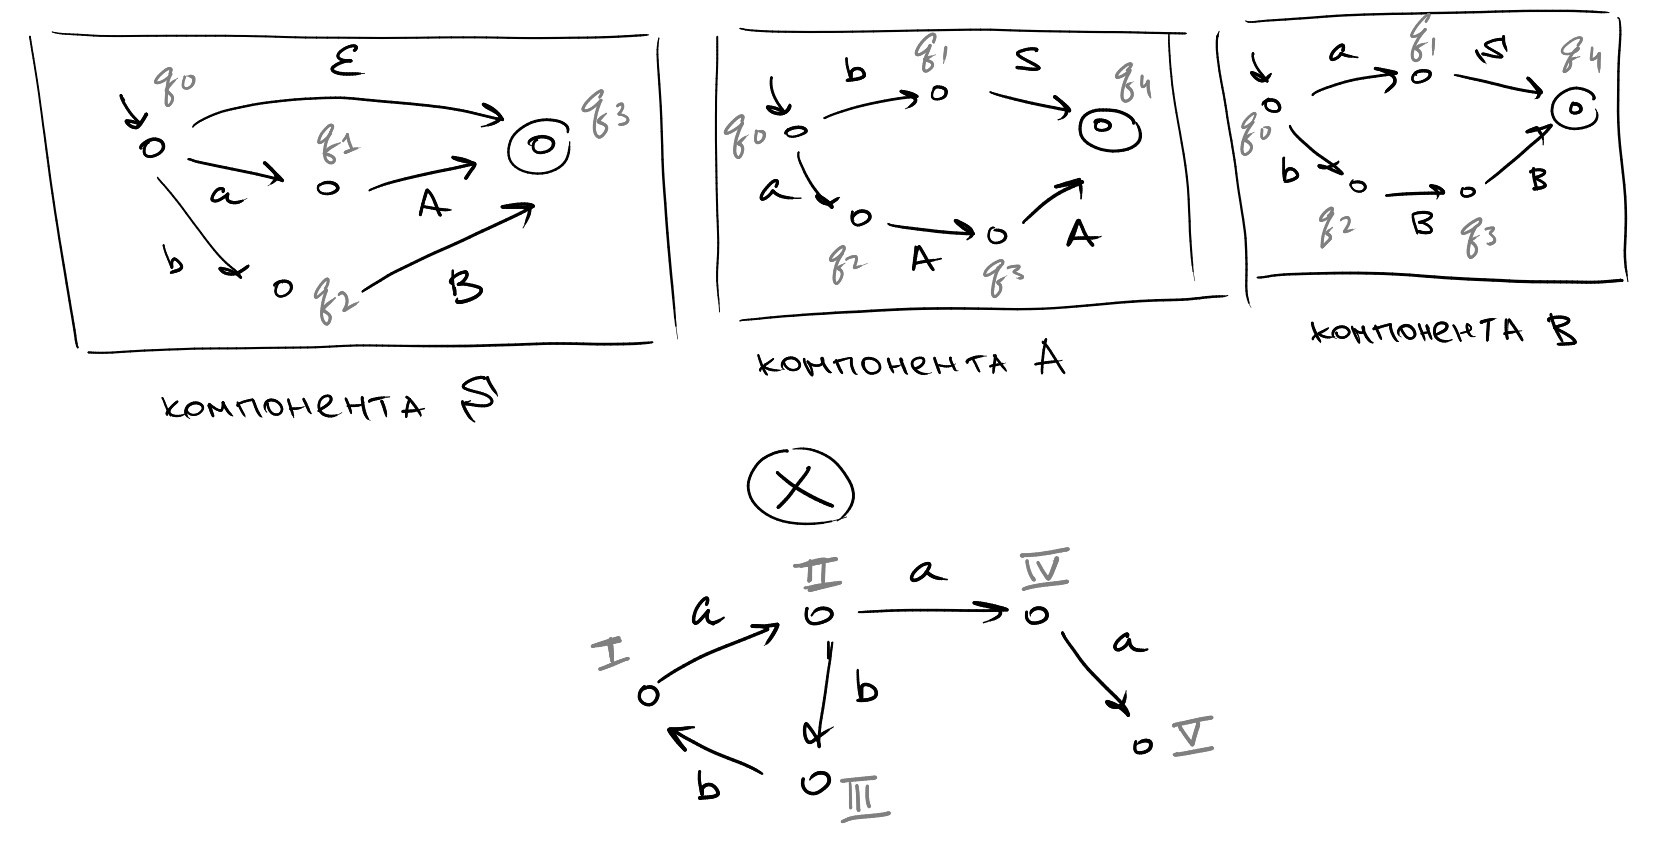
\includegraphics[width=1\linewidth]{img/example_intersection1}

%     \TODO: дорисовать пример (а потом перерисовать)

% \end{example}

Для проверки непустоты получившегося языка, нужно проверить, существует ли путь из стартового состояния $\q{q_s, u}$ в конечное состояние $\q{q_t, v}$ ($q_s$ и $q_t$ принадлежат начальной компоненте). То есть решить задачу достижимости для РКА.

Как будет обсуждено позже, при решении задачи достижимости для РКА, строится матрица достижимости (т.е. для каждой пары состояний находится, есть ли путь из одного в другое). Так что за один запуск такого алгоритма можно проверить КС-достижимость для всех пар вершин исходного графа. 
% нужно решить задачу достижимости на построенном РКА-произведении.

Подводя итог, все алгоритмы для CFPQ, основанные на идее пересечения языков, будут иметь следующую схему:
\begin{enumerate}
    \item Построить прямое произведение входной грамматики $\cool{R}$ и входного графа $G$: $\cool{P} = \cool{R} \otimes G$.
    \item \textit{Решить задачу достижимости для полученного РКА $\cool{P}$}
    \item Из вершины $u$ в вершину $v$ входного графа существует путь, выводимой входной грамматикой $\cool{G}$ $\EQ$ в $\cool{P}$ есть путь $(q_0, u) \path (q_f, v)$ из стартового в конечное состояние начальной компоненты РКА $\cool{P}$
\end{enumerate}

Второй пункт~--- решение задачи достижимости для РКА~--- будет подробно рассмотрен далее.

\subsection{Решение задачи достижимости для РКА}

Решение задачи достижимости для НКА эквивалентно~\cite{Yannakakis1990} решению задачи достижимости для обычного ориентированного графа и заключается в построении транзитивного замыкания.

% Транзитивное замыкание
\begin{definition}\label{def:TC}
  \TODO
\end{definition}

В случае РКА же всё сложнее~--- про часть рёбер (все рекурсивные рёбра) непонятно, присутствуют ли они в графе. А именно, рекурсивное ребро $u \xrightarrow{en, ex} v$ присутствует (может быть использовано для построения путей) только если состояние $ex$ достижимо из состояния $en$.

Для обработки таких ситуаций задачу решают итеративно: при обнаружении достижимости пары вершин проводят новые рёбра (рекурсивные рёбра с соответствующей меткой) и обновляют отношение достижимости (после этого могут появиться новые рёбра, которые снова проводят, и так далее). Такая задача уже сводится к решению задачи поддержания {\bf инкрементального} транзитивного замыкания.

% Инкрементальное транзитивное замыкание
\begin{definition}
  \TODO
\end{definition}

В листинге~\ref{algo:PI} приведён псевдокод алгоритма решения задачи достижимости для РКА, основанный на поддержании инкрементального транзитивного замыкания.

\begin{note}
  Отдельно, до начала основного алгоритма, нужно обработать $\eps$-переходы. Эта часть алгоритма опущена (здесь и далее) для простоты изложения. 
\end{note}

\begin{algorithm}[h]
    \floatname{algorithm}{Listing}
    \begin{algorithmic}[1]
    \caption{Алгоритм достижимости для РКА}
    \label{algo:PI}
    \Function{RSMReachability2}{$\cool{R}$}
        \State{$A \gets$ Empty adjacency matrix}
        \State{$Q \gets$ Empty Queue}
        \For{$i \in 1..k$}
            \For{$u \xrightarrow{c} v \in \delta_i$}
                \State{$Q.Push(\q{u, v, i})$}
            \EndFor
        \EndFor
        \While{$Q$ is not Empty}
            \State{$\q{u, v, i} \gets Q.Pop()$}
            \If{$u \in En_i \wedge v \in En_i$}
                \Comment{Нашли новый путь}
                \State{$A \gets A \cup getEdges(i, u, v)$}
                \State{$Q.PushAll(getEdges(i, u, v))$}
                \Comment{Добавляем новые рёбра}
            \EndIf
            \For{$x \in Q_i$}
                \If{$A_{x, u} \wedge \overline{A_{x, v}}$}
                    \For{$y \in Q_i$} 
                        \If{$A_{v, y} \wedge \overline{A_{x, y}}$}
                            \State{$A \gets A \cup \q{x, y}$}
                            \State{$Q.Push(\q{x, y, i})$}
                            \Comment{Обновлем транзитивное замыкание}
                        \EndIf
                    \EndFor
                \EndIf
            \EndFor
        \EndWhile
    \State \Return $A$
    \EndFunction
    \end{algorithmic}
\end{algorithm}

Работа происходит над матрицей смежности $\cool{R}$~--- изначально туда записываются все внутренние (нерекурсивные) рёбра. 

В алгоритме используется стандартная реализация инкрементального транзитивного замыкания~\cite{Ibaraki1983}. Для этого в ходе работы алгоритма поддерживается рабочая очередь $Q$ рёбер транзитивного замыкания, которые были найдены, но ещё не обработаны. 

При обработке очередного ребра, ищутся новые пути, которые проходя через него. А именно, пусть было добавлено ребро $u \to v$. Тогда далее перебирается вершина $x$, такая что из неё была достижима вершина $u$ ($x \path u$), но не была достижима вершина $v$ ($x \not\path v$). Из такой вершины $x$ становятся достижимы все вершины $y$, которые были достижимы из $v$ ($v \path y$).

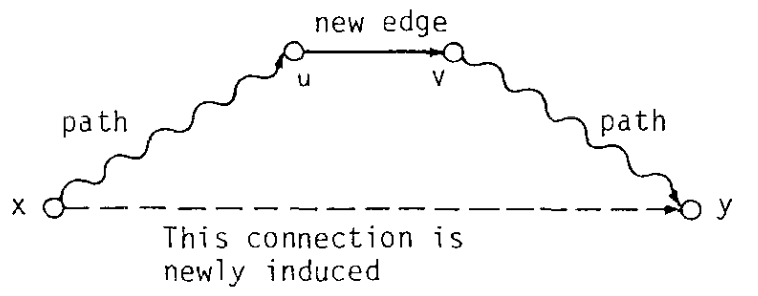
\includegraphics[width=0.75\linewidth]{img/TC_add}

\TODO: норм картинка

Если новое ребро ТЗ (= путь в графе) соединяет начальную и конечную вершину, в очередь добавляются также все соответствующие ему рекурсивные рёбра: для нового пути $(en \in En_i) \path (ex \in Ex_i)$ проводятся все рёбра, соответствующие рекурсивным вызовам $i$-ой компоненты с начальной вершиной $en$ и конечной вершиной $ex$.

\subsubsection*{Время работы}

Внешний цикл итерируется по всем рёбрам, так что работает за $\O(|E^{*}|)$ (где $E^{*}$~--- рёбра итогового транзитивного замыкания). Добавление новых рёбер рассмотрит каждое ребро не более одного раза, так что тоже работает за $O(|E^{*}|)$. Нужно только оценить работу по поддержанию транзитивного замыкания. 

Цикл на строке 12 перебирает все вершины, так что отработает суммарно за $\O(|E^{*}| |V|)$. Внутренний цикл (строка 14) тоже перебирает все вершины, но после его выполнения будет добавлено хотя бы одно новое ребро ($x \to v$), так что суммарное время работы этих циклов также можно оценить как $\O(|E^{*}| |V|)$.

Итого, суммарное время работы составляет $\O(|E^{*}||V|)$, что в плотных графах будет равно $\Theta(|V|^3)$. 

\begin{note}
  Время работы инкрементального транзитивного замыкания можно ускорить в $\log |V|$ раз~\cite{Shemetova21}, воспользовавшись методом четырёх русских~\cite{Arlazarov70} (так как работа происходит над булевыми векторами).
\end{note}

\subsection{Получение решений для частных случаев}

Основой для получения частных решений будут модификации данного алгоритма~\ref{algo:PI}.

Как уже было сказано, узким местом алгоритма является поддержание инкрементального транзитивного замыкания. На его время работы (так же, как и на время работы задачи CFPQ) существует кубическая условная нижняя оценка: к ней сводится~\cite{Henzinger15} задача \s{OMv}\footnote{Online Matrix-Vector Multiplication~--- онлайн умножения матрицы и векторов}. 

Следовательно, чтобы получить более быстрые алгоритмы, нужно рассматривать такие частные случаи, для которых задачу инкрементального транзитивного замыкания можно решать за субкубическое время.

Опишем такие случаи:

\begin{itemize}
  \item \textit{Графы с ограниченной степенью}

    В~\cite{Yellin1993} представлен алгоритм для инкрементального транзитивного замыкания на графах с ограниченной исходящей степенью. Асимптотика алгоритма: $\O(d |E^{*}|)$, где $d$~--- ограничение сверху на исходящую степень графа.

  \item \textit{Планарные графы}

    \TODO: Разобраться, что там написано у Александры 
  
  \item \textit{Автоматы, с ограниченным стеком\footnote{Bounded-stack State Machines}~\cite{Chaudhuri08}}

    Для автоматов, РКА которых не уходит в рекурсию, был построен~\cite{Chaudhuri08} алгоритм, с временем работы $\O(|V|^3 / \log^2 |V|)$.

  \item \textit{Неориентированные графы}

    Подробнее рассмотрены в главе~\ref{section:bidirected}

  \item \textit{\TODO: ???}
    
    Подробно рассмотрены в главе~\ref{section:dyck_1}

\end{itemize}

\subsection{Выводы и результаты по главе}


\includegraphics[width=0.75\linewidth]{img/conclusion_cat}

\TODO